\section{Calculations and Results}
From the following equaitions,

$$ \tau_z = I\beta_z $$
$$ I_{ab} = I_A + I_B $$
$$ M_\mu = -I_1\beta_1 $$
$$ T = m(g-a)$$

We can derive
$$ m(g-R\beta_2)R-M_\mu=I_1\beta_2 $$
Then we find
$$ I_1=\frac{mR(g-R\beta_2)}{\beta_2-\beta_1} $$
Similarly, if a rigid body with an unknown moment of inertia is placed on the
turntable, we may find 
$$ I_2=\frac{mR(g-R\beta_4)}{\beta_4-\beta_3} $$
Using the fact that the moment of inertia is an additive quantity, the moment of
inertia of the rigid object placed on the turntable, with respect to the axis of
rotation, may be found as the difference 
$$ I_3 = I_2 - I_1 $$

\subsection{Measurement of Angular Acceleration}
Angular acceleration can be derive by investigating the measurement data (k,t),
the corresponding angular position is
$$ \theta = k\pi = \omega_0 t + \frac{1}{2}\beta t^2 $$


\subsection{In Lab Data}

\begin{table}[H]
  \centering
  \begin{tabularx}{\textwidth}{|p{6cm}|X|X|X|X|}
    \hline
    Object & 1 & 2 & 3 & 4 \\
    \hline
    Disk $[cm] \pm 0.002[cm]$& 24.098 & 24.094 & 24.094 & 24.094 \\
    Hoop 1 $[cm] \pm 0.002[cm]$& 20.982 & 20.918 & 20.966 & 20.976 \\
    Hoop 2 $[cm] \pm 0.002[cm]$& 23.998 & 24.000 & 24.000 & 24.002 \\
    Cylinder A $[cm] \pm 0.002[cm]$& 2.994 & 2.994 & 2.994 & 2.994 \\
    Cylinder B $[cm] \pm 0.002[cm]$& 2.994 & 2.994 & 2.994 & 2.994 \\
    Cone pulley $[cm] \pm 0.002[cm]$& 5.022 & 5.020 & 5.008 & 5.008 \\
    Hole 1 d $[cm] \pm 0.002[cm]$& 3.978 & 5.534 & & \\
    Hole 2 d $[cm] \pm 0.002[cm]$& 3.982 & 5.540 & & \\
    Hole 3 d $[cm] \pm 0.002[cm]$& 5.524 & 6.500 & & \\
    Hole 4 d $[cm] \pm 0.002[cm]$& 5.520 & 6.520 & & \\
    \hline
  \end{tabularx}
  \caption{Calliper measurements}
  \end{table}


\begin{table}[H]
  \centering
  \begin{tabularx}{\textwidth}{|X|X|}
    \hline
    Object & Mass\\
	\hline
    Disk $[g] \pm 0.1 [g] $ & 493.1\\
    Hoop $[g] \pm 0.1 [g] $ & 422.5\\
    Cylinder A $[g] \pm 0.1 [g] $ & 165.8\\
    Cylinder B $[g] \pm 0.1 [g] $ & 165.8\\
    Weight $[g] \pm 0.1 [g] $ & 59.1 \\
    \hline
  \end{tabularx}
  \caption{Mass measurements}
  \end{table}
% begin real data
\begin{table}[H]
  \centering
\begin{tabular}{|p{2cm}|p{1.5cm}|l|l|l|l|l|l|l|l|l|}
\hline
Situation & A or D & k & 1 & 2 & 3 & 4 & 5 & 6 & 7 & 8 \\
\hline
Empty & Dec & $t[s]$ & 0.2958 & 0.5924 & 0.8899 & 1.1881 & 1.4873 & 1.7871 & 2.0879 & 2.3895 \\
Empty & Acc & $t[s]$ & 0.9005 & 1.5186 & 2.0204 & 2.4557 & 2.8448 & 3.1996 & 3.5280 & 3.7038 \\
With disk & Dec &  $t[s]$ & 0.3178 & 0.6362 & 0.9554 & 1.2752 & 1.5958 & 1.9170 & 2.2390 & 2.5616 \\
With disk & Acc &  $t[s]$ & 0.8957 & 1.5808 & 2.1582 & 2.6666 & 3.1264 & 3.5491 & 3.9428 & 4.3322 \\
With hoop & Dec &  $t[s]$ & 0.2450 & 0.4903 & 0.7359 & 0.9818 & 1.2281 & 1.4746 & 1.7216 & 1.9688 \\
With hoop & Acc &  $t[s]$ & 1.0035 & 1.7614 & 2.3967 & 2.9547 & 3.4589 & 3.9216 & 4.3521 & 4.7560 \\
A 1 B 2 & Dec &  $t[s]$ & 0.4491 & 0.9003 & 1.3536 & 1.8089 & 2.2666 & 2.7263 & 3.1883 & 3.6524 \\
A 1 B 2 & Acc &  $t[s]$ & 1.3586 & 2.0905 & 2.6595 & 3.1424 & 3.5692 & 3.9562 & 4.3125 & 4.6448 \\
A 3 B 4 & Dec &  $t[s]$ & 0.4539 & 0.9099 & 1.3678 & 1.8279 & 2.2899 & 2.7541 & 3.2204 & 3.6888 \\
A 3 B 4 & Acc &  $t[s]$ & 1.3748 & 2.1298 & 2.7179 & 3.2171 & 3.6585 & 4.0587 & 4.4273 & 4.7711 \\
\hline
\end{tabular}
\caption{ Time measurements}
\end{table}

According to  United States Department of Commerce, the standard gravitational
acceleration is 
$$ g =  9.80665 m/s^2 $$


For the Empty turntable,
\newcommand{\EFWwr}{17cm}
\begin{figure}[H]
\centering
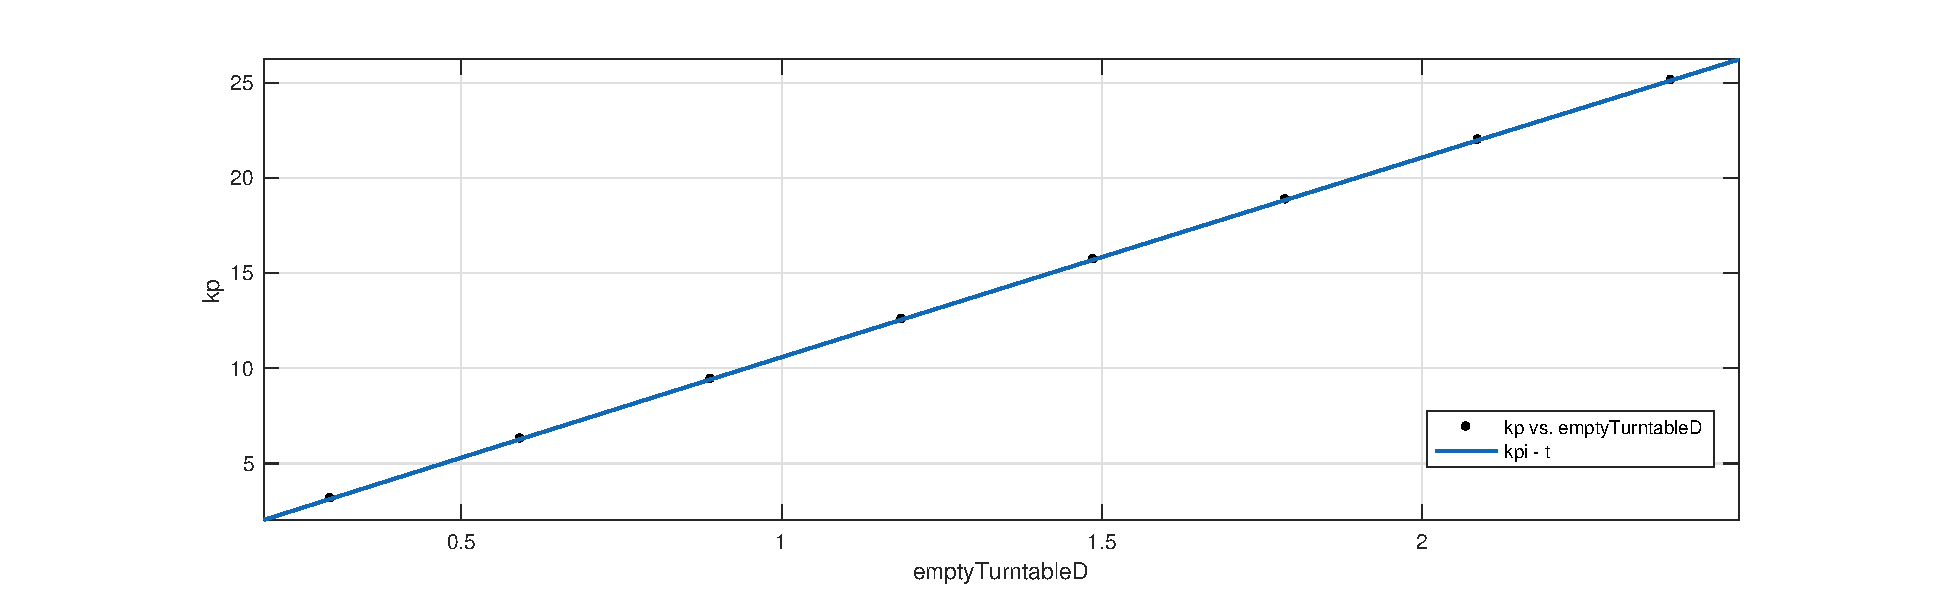
\includegraphics[width=\EFWwr]{matlab/etd}
\end{figure}

$$ \beta_1 = -0.0970 radius/s^2$$ (with 95\% confidence bounds) 

\begin{figure}[H]
\centering
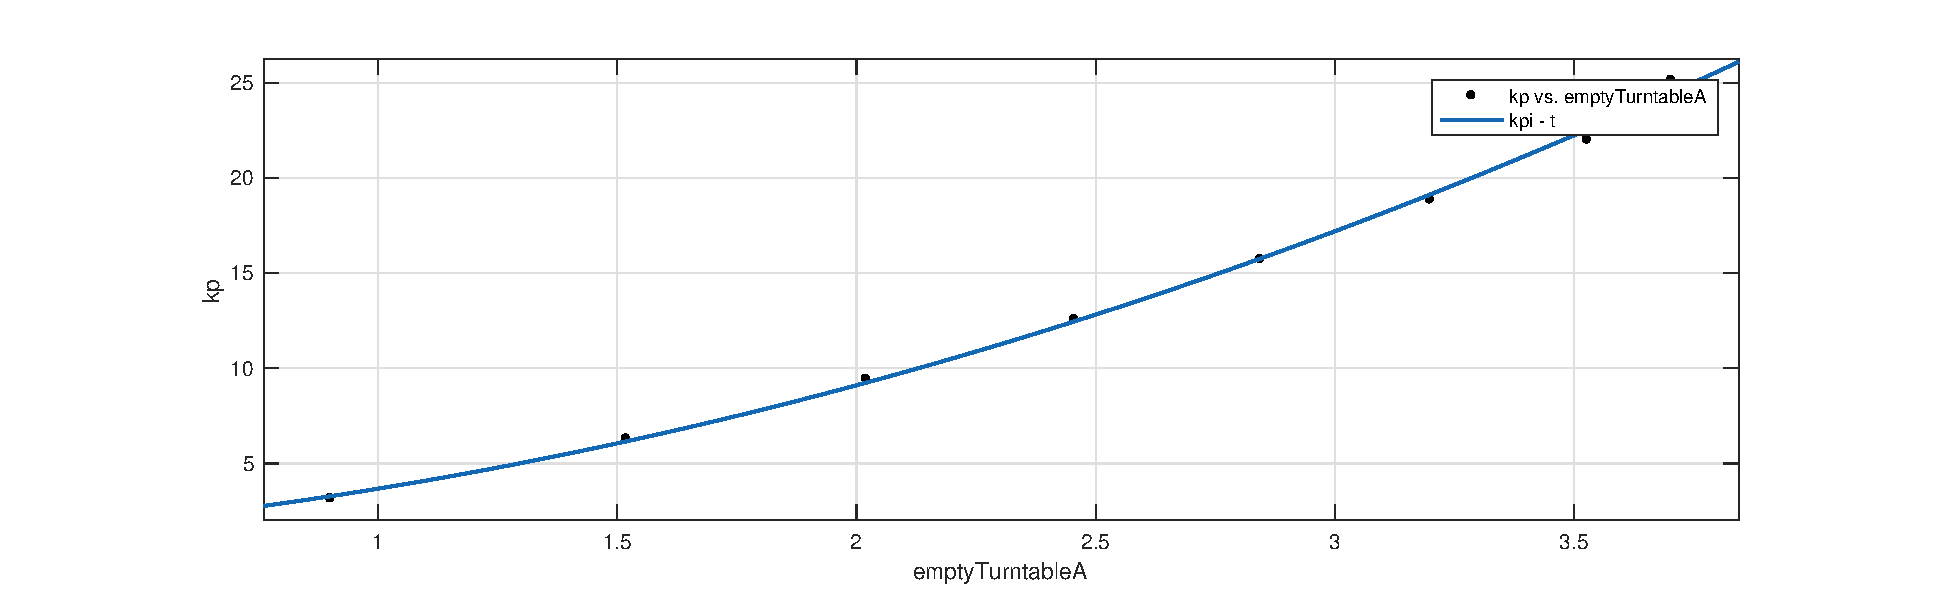
\includegraphics[width=\EFWwr]{matlab/eta}
\end{figure}

$$ \beta_2 = 2.6580 radius/s^2$$ (with 95\% confidence bounds) 

Thus,
$$ I_1 = \frac{59.1 g \times 5.0145 cm \times (9.80665 m/s^2 - 5.0145 cm \times (-0.0970) radius/s^2 )}{2.6580 radius/s^2 -(-0.0970 radius/s^2) } = 0.0105 kg\times m^2 $$

For turntable with disk 
\begin{figure}[H]
\centering
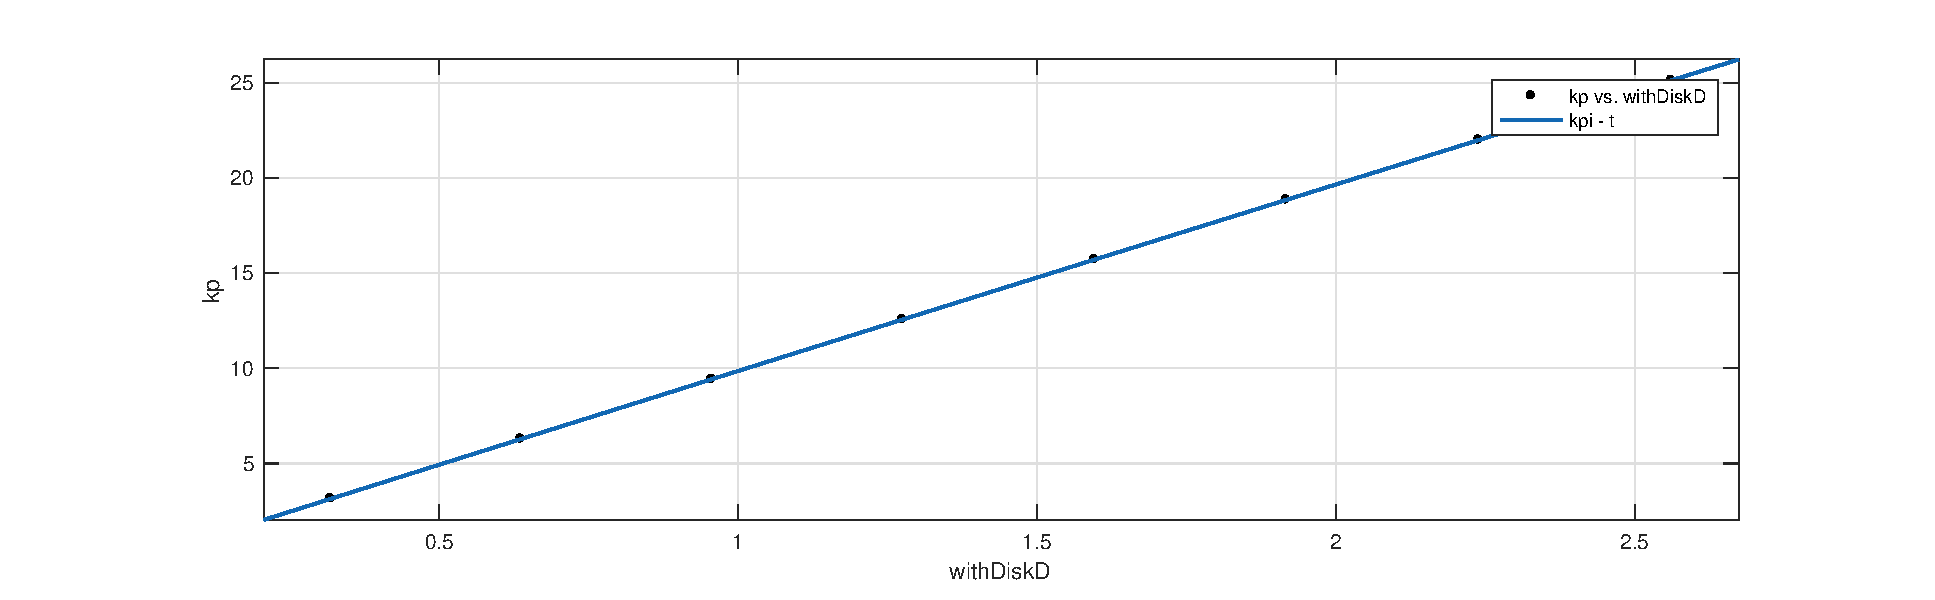
\includegraphics[width=\EFWwr]{matlab/wdd}
\end{figure}

$$ \beta_1 = -0.0668 radius/s^2$$ (with 95\% confidence bounds) 

\begin{figure}[H]
\centering
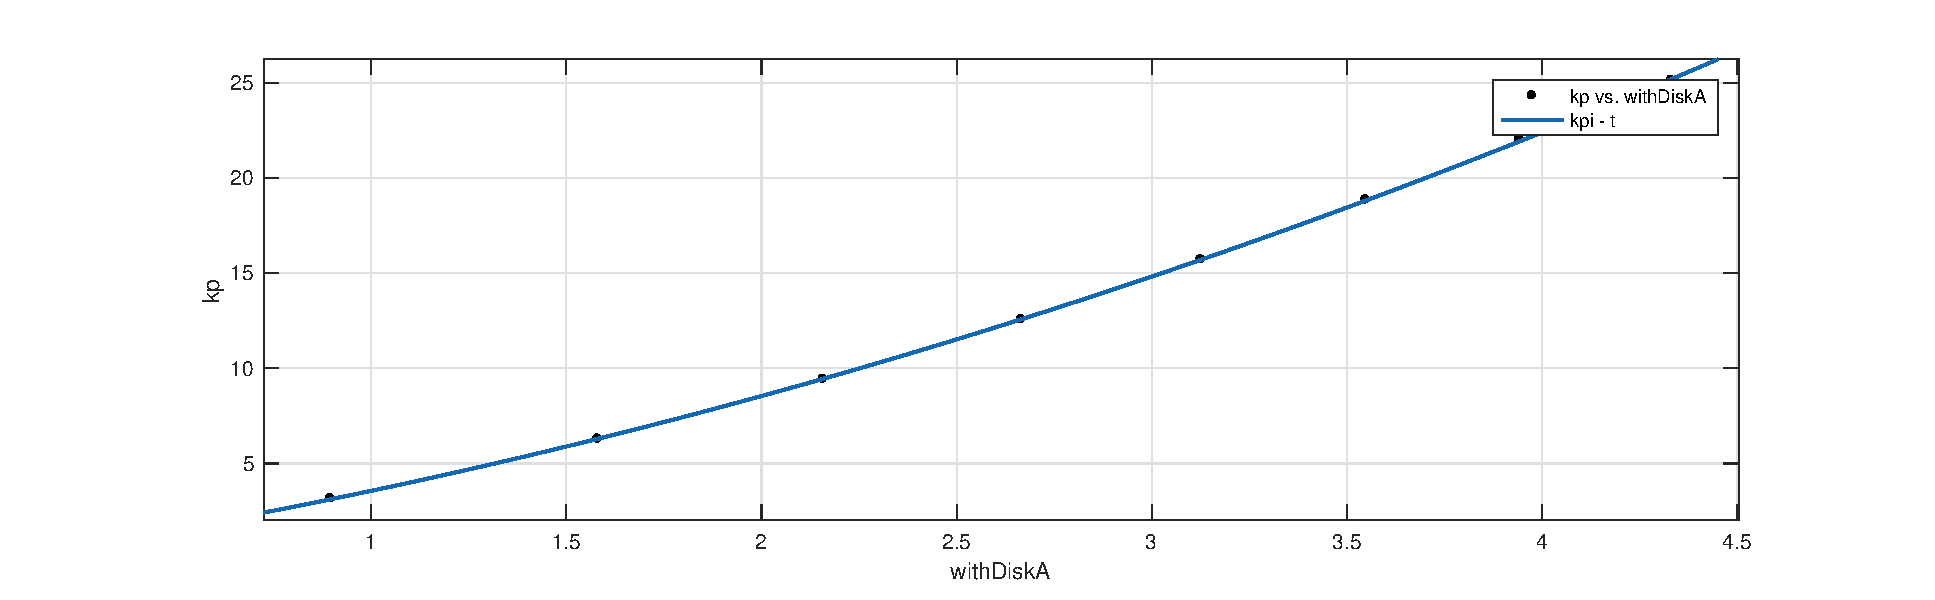
\includegraphics[width=\EFWwr]{matlab/wda}
\end{figure}

$$ \beta_2 = 1.2970 radius/s^2$$ (with 95\% confidence bounds) 

$$ I_2 = \frac{59.1 g \times 5.0145 cm \times (9.80665 m/s^2 - 5.0145 cm \times (-0.0668) radius/s^2 )}{1.2970 radius/s^2 -(-0.0668 radius/s^2) } = 0.0213 kg\times m^2 $$


% ======

-0.0689
1.1444

-0.0710
1.8752

-0.0661
1.7496


$$ \beta_1 = -0.0668 radius/s^2$$ (with 95\% confidence bounds) 

\begin{figure}[H]
\centering
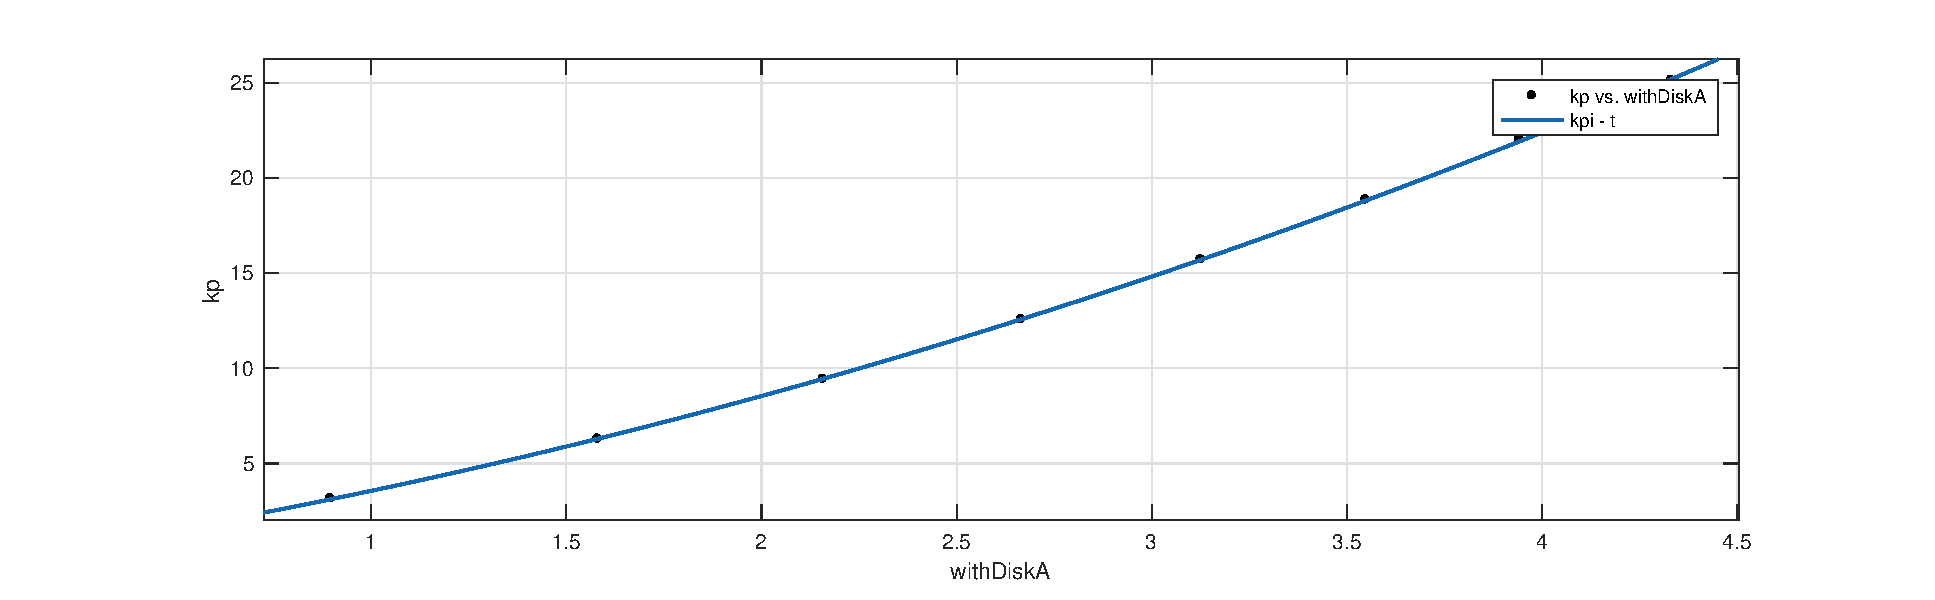
\includegraphics[width=\EFWwr]{matlab/wda}
\end{figure}

$$ \beta_2 = 1.2970 radius/s^2$$ (with 95\% confidence bounds) 

$$ I_2 = \frac{59.1 g \times 5.0145 cm \times (9.80665 m/s^2 - 5.0145 cm \times (-0.0668) radius/s^2 )}{1.2970 radius/s^2 -(-0.0668 radius/s^2) } = 0.0213 kg\times m^2 $$$$ \beta_1 = -0.0668 radius/s^2$$ (with 95\% confidence bounds) 

\begin{figure}[H]
\centering
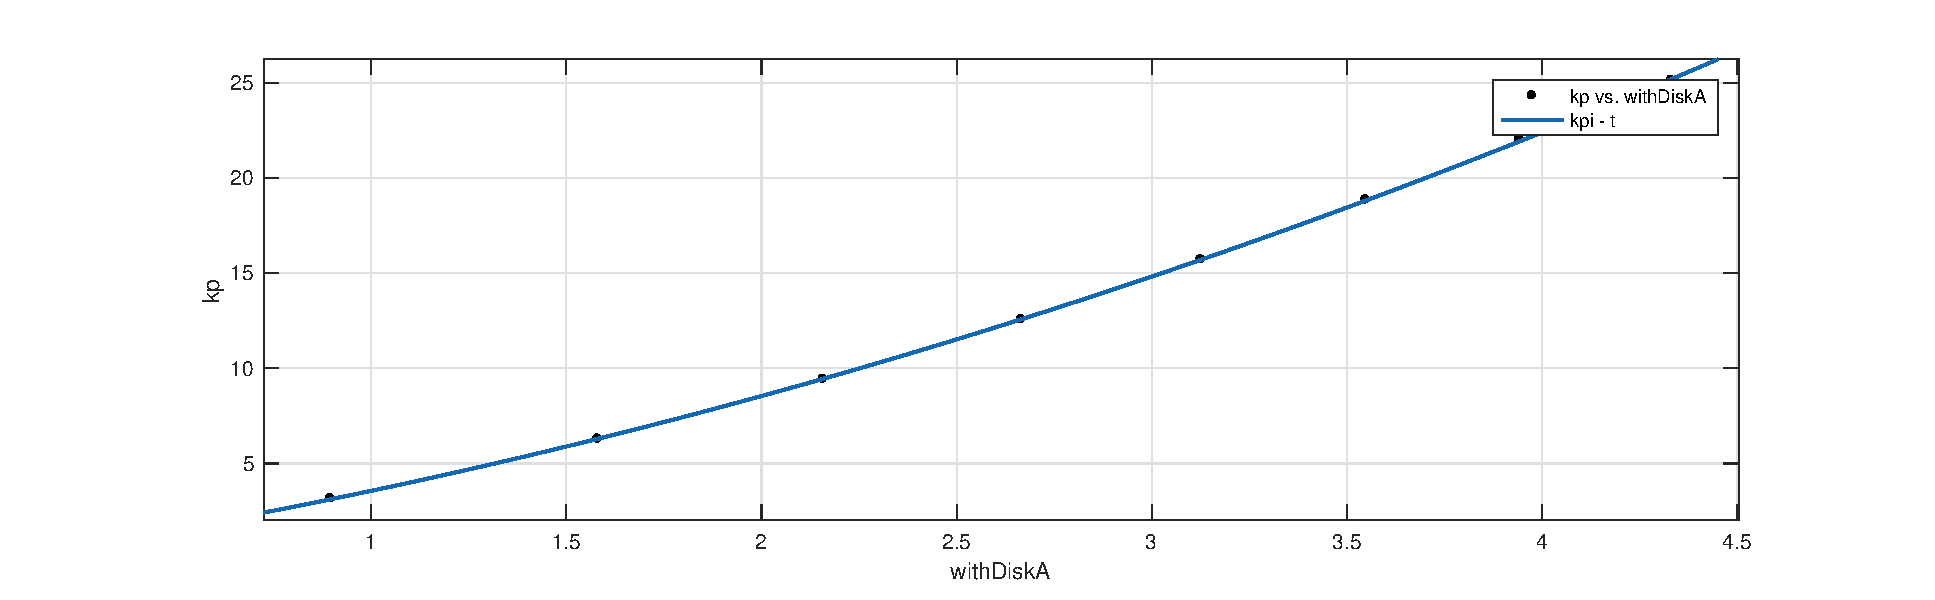
\includegraphics[width=\EFWwr]{matlab/wda}
\end{figure}

$$ \beta_2 = 1.2970 radius/s^2$$ (with 95\% confidence bounds) 

$$ I_2 = \frac{59.1 g \times 5.0145 cm \times (9.80665 m/s^2 - 5.0145 cm \times (-0.0668) radius/s^2 )}{1.2970 radius/s^2 -(-0.0668 radius/s^2) } = 0.0213 kg\times m^2 $$$$ \beta_1 = -0.0668 radius/s^2$$ (with 95\% confidence bounds) 

\begin{figure}[H]
\centering
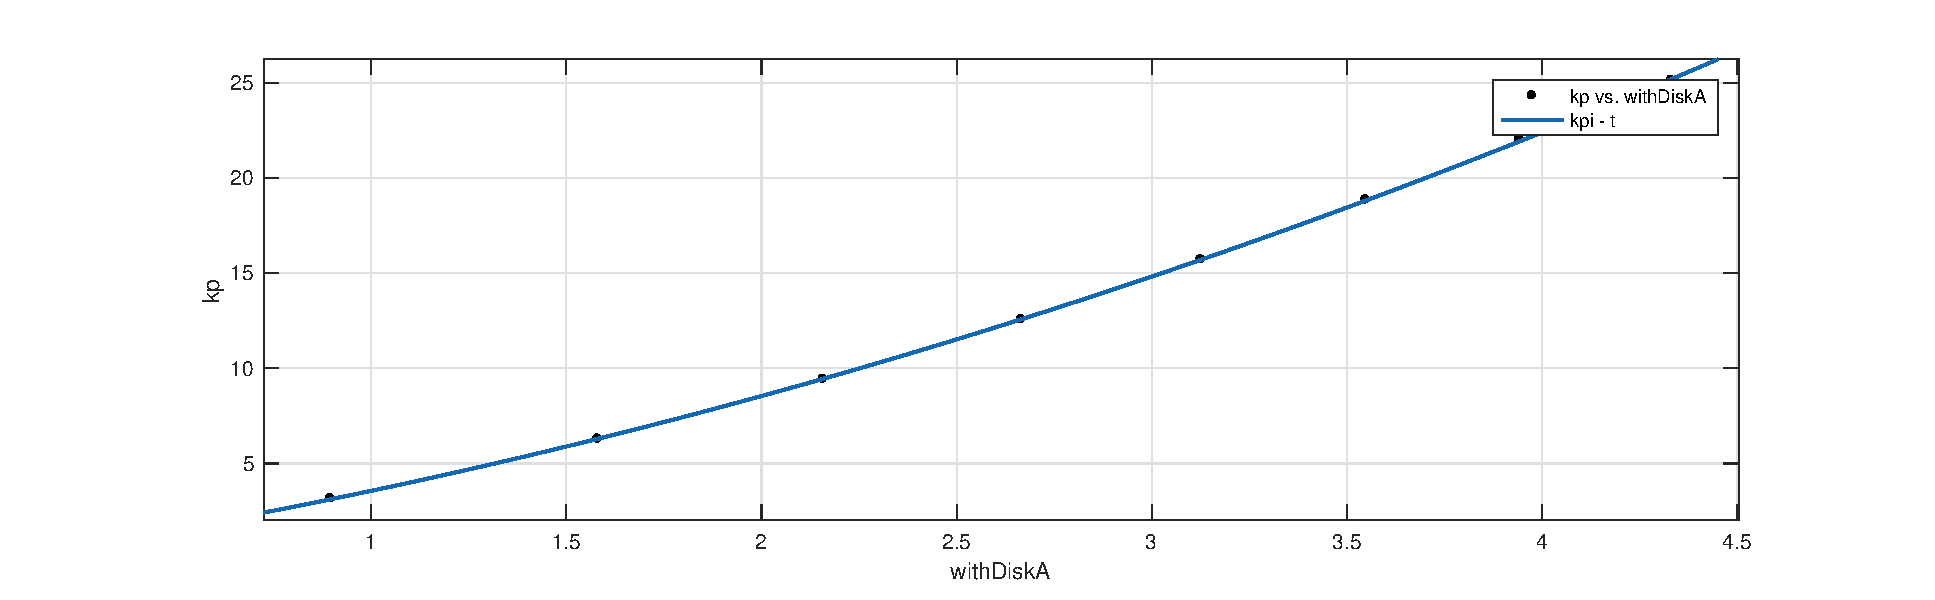
\includegraphics[width=\EFWwr]{matlab/wda}
\end{figure}

$$ \beta_2 = 1.2970 radius/s^2$$ (with 95\% confidence bounds) 

$$ I_2 = \frac{59.1 g \times 5.0145 cm \times (9.80665 m/s^2 - 5.0145 cm \times (-0.0668) radius/s^2 )}{1.2970 radius/s^2 -(-0.0668 radius/s^2) } = 0.0213 kg\times m^2 $$$$ \beta_1 = -0.0668 radius/s^2$$ (with 95\% confidence bounds) 

\begin{figure}[H]
\centering
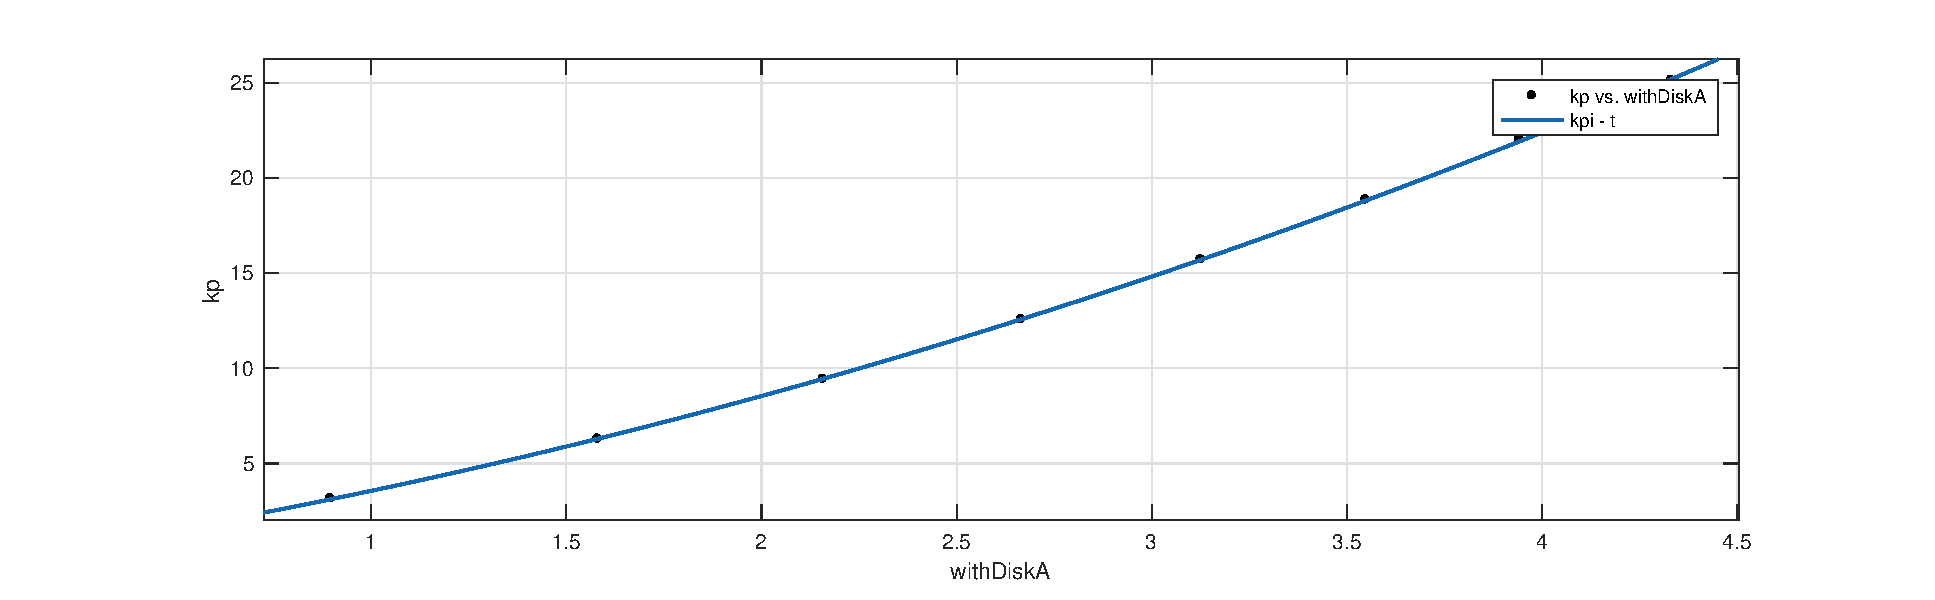
\includegraphics[width=\EFWwr]{matlab/wda}
\end{figure}

$$ \beta_2 = 1.2970 radius/s^2$$ (with 95\% confidence bounds) 

$$ I_2 = \frac{59.1 g \times 5.0145 cm \times (9.80665 m/s^2 - 5.0145 cm \times (-0.0668) radius/s^2 )}{1.2970 radius/s^2 -(-0.0668 radius/s^2) } = 0.0213 kg\times m^2 $$$$ \beta_1 = -0.0668 radius/s^2$$ (with 95\% confidence bounds) 

\begin{figure}[H]
\centering
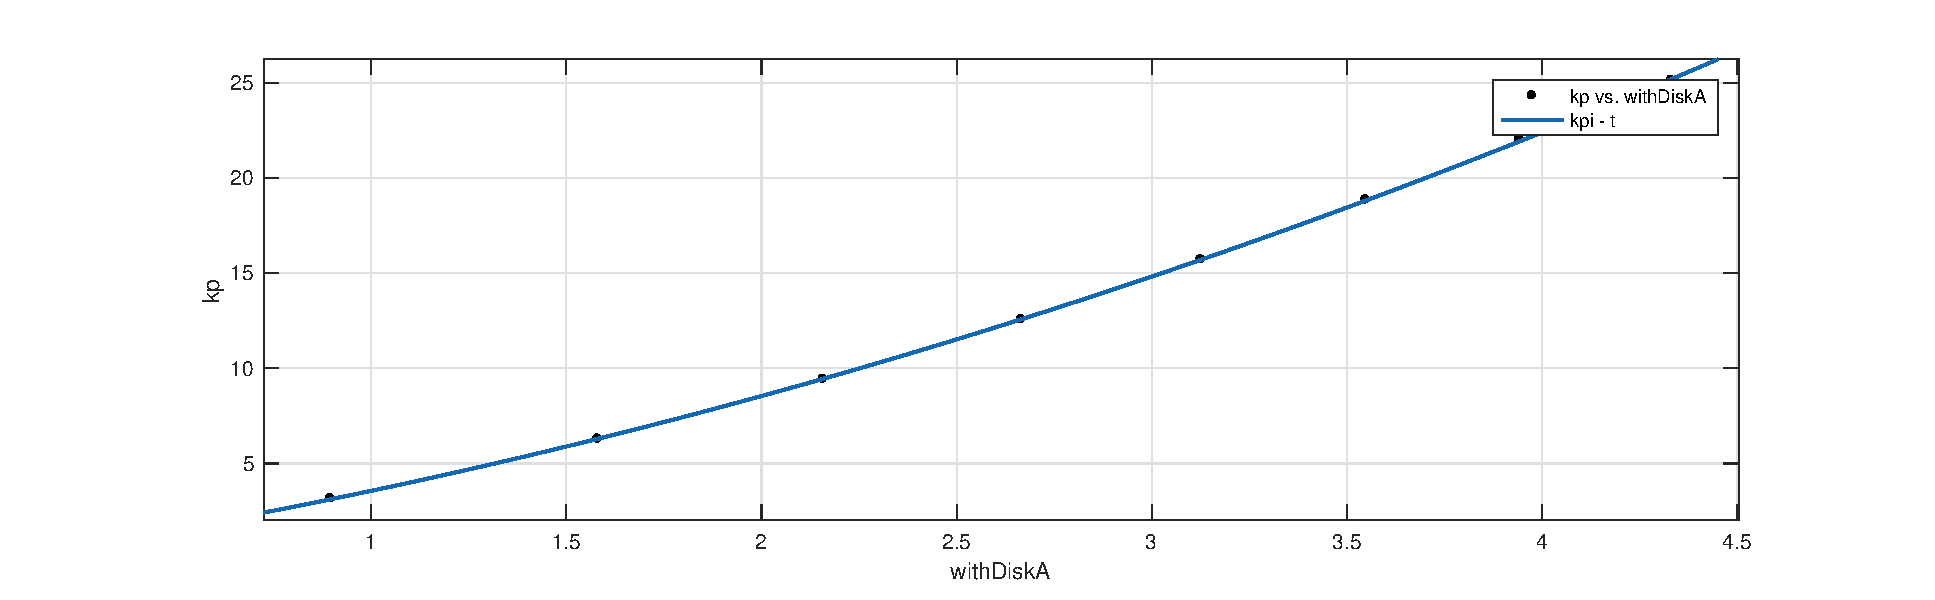
\includegraphics[width=\EFWwr]{matlab/wda}
\end{figure}

$$ \beta_2 = 1.2970 radius/s^2$$ (with 95\% confidence bounds) 

$$ I_2 = \frac{59.1 g \times 5.0145 cm \times (9.80665 m/s^2 - 5.0145 cm \times (-0.0668) radius/s^2 )}{1.2970 radius/s^2 -(-0.0668 radius/s^2) } = 0.0213 kg\times m^2 $$$$ \beta_1 = -0.0668 radius/s^2$$ (with 95\% confidence bounds) 

\begin{figure}[H]
\centering
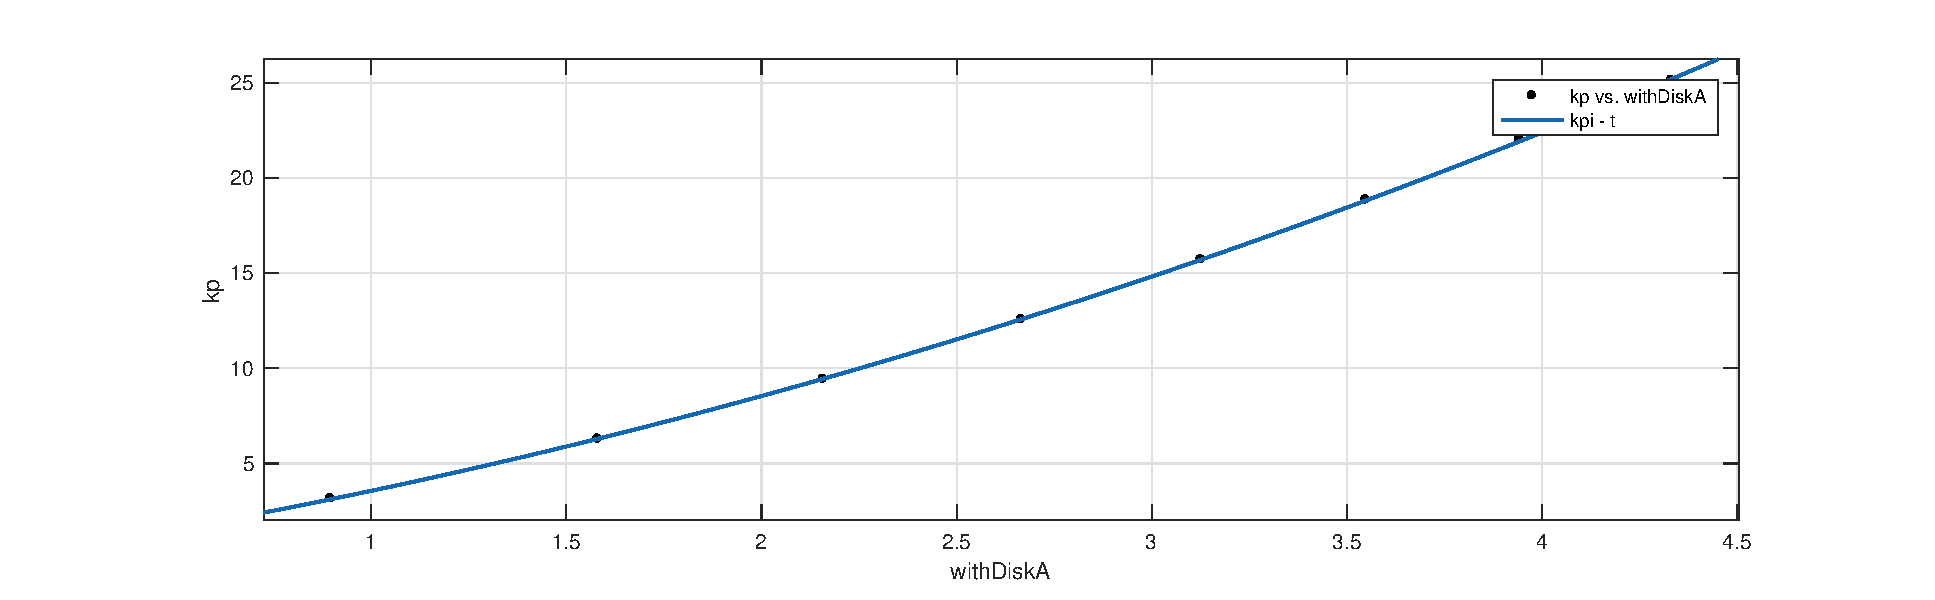
\includegraphics[width=\EFWwr]{matlab/wda}
\end{figure}

$$ \beta_2 = 1.2970 radius/s^2$$ (with 95\% confidence bounds) 

$$ I_2 = \frac{59.1 g \times 5.0145 cm \times (9.80665 m/s^2 - 5.0145 cm \times (-0.0668) radius/s^2 )}{1.2970 radius/s^2 -(-0.0668 radius/s^2) } = 0.0213 kg\times m^2 $$

 

